\documentclass{book}

\usepackage[utf8]{inputenc}
\usepackage{graphicx}
\usepackage[section]{placeins}
\usepackage[
bookmarks=true,
colorlinks=true,
breaklinks=true,
urlcolor=red,
citecolor=blue,
linkcolor=black,
unicode=true,
]
{hyperref}

\begin{document}
\title{Algoritmizace Hashing}
\maketitle
Hashovací tabulky jsou datové struktury, které používají hashovací funkci k vyhledávání dat. Hashovací funkce $h(k)$ zobrazuje množinu klíčů $k$ do intervalu adres $\langle a_{min}, a_{max}\rangle$.

\begin{itemize}
\item Volba hashovací funkce pro celá čísla:
\begin{itemize}
\item Multiplikativní (m je prvočíslo)
\begin{equation}
h(k) = round(\frac{k}{2^w\cdot m})
\end{equation}
\item Modulární
\begin{equation}
h(k) = k \% n
\end{equation}
\item Kombinovaná
\begin{equation}
h(k) = round(c\cdot k)\% m, c \in \langle 0, 1 \rangle 
\end{equation}
\end{itemize}
\item Pro řetězce: 
\begin{itemize}
\item Hornerovo schéma
\begin{equation}
h(k) = k_n \cdot a^n + ... + k_0 \cdot a^0
\end{equation}
\end{itemize}
\end{itemize}

\section{Řešení kolizí}

Kolize vzniká když $h(k)$ vrací pro různé klíče stejnou hodnotu.

\subsection{Hashování se separovanými řetězci}
Hlavní myšlenka je, že pro každou možnou adresu vytvoříme spojový seznam a do něj přidáváme všechny prvky s danou adresou. Demonstrace v \ref{fig:strings}.

\begin{itemize}
\item{Výhody}
\begin{itemize}
\item Nemusíme znát předem počet prvků
\end{itemize}
\item Nevýhody
\begin{itemize}
\item Potřebujeme dynamické přidělování paměti
\item Potřebuje navíc paměť na ukazatele a na tabulku (heads v Figure \ref{fig:strings})
\end{itemize}
\end{itemize}

Složitost operací:
\begin{itemize}
\item Vkládání $O(1)$ (nebo složitost vložení do struktury kterou používáme místo spojového seznamu)
\item Vyhledání $O(n)$ (nejhorší případ kdy jsou všechny prvky v kolizi)
\end{itemize}

\subsection{Otevřené hashování}
Hlavní myšlenka je, že pokud mám zhruba odhad počtu prvků které budu vkládat, tak mohu ušetřit na zbytečném ukládání ukazatelů tím, že budu ukládat kolize rovnou do tabulky. To může být provedeno následujícími způsoby:
\begin{itemize}
\item Lineární přidávání (když nastane kolize prvek se vloží na další volnou pozici). Demonstrace v Figure \ref{fig:linear_probing}.

Složitost operací:
\begin{itemize}
\item Vkládání $O(n)$ (nejhorší případ kdy jsou všechny prvky v kolizi)
\item Vyhledání $O(n)$ (nejhorší případ kdy jsou všechny prvky v kolizi)
\end{itemize}

\item Dvojité hashování (když nastane kolize použije se druhá hashovací funkce, pomocí níž se spočítá offset a prvek se vloží na pozici kam měl být dán + offset). Demonstrace v Figure \ref{fig:double_hashing}.

Složitost operací:
\begin{itemize}
\item Vkládání $O(n)$ (nejhorší případ kdy jsou všechny prvky v kolizi v první i druhé hash funkci)
\item Vyhledání $O(n)$ (nejhorší případ kdy jsou všechny prvky v kolizi v první i druhé hash funkci)
\end{itemize}

\end{itemize}

\subsection{Srůstající hashování}
Hlavní myšlenka je omezení clusterování otevřeného hashování přidáním ukazatele pro každý prvek v tabulce. Možnosti provedení:
\begin{itemize}
\item Bez pomocné paměti (prvky se vkládají na pozice v tabulce)
\begin{itemize}
\item LISCH (late insert standard coalesced hashing)
\item EISCH (early insert standard coalesced hashing)
\end{itemize}
\item S pomocnou pamětí (prvky se vkládají na k tomu určené místo tzv. sklep za adresovým prostorem tabulky)
\begin{itemize}
\item LICH (late insert coalesced hashing)
\item EICH (early insert coalesced hashing)
\item VICH (variable insert coalesced hashing)
\end{itemize}
\end{itemize}

\subsubsection{LISCH}
Přidává myšlenku ukazatele na poslední volné místo v tabulce (inicializován na poslední pozici). Při kolizi se prvek přidá na místo kam ukazuje tento ukazatel a ukazatel se opět přesune na poslední volné místo. Prvek na pozici kde vznikla kolize si drží ukazatel na pozici kam byl vložen kolidující prvek, ten si zase drží odkaz na další prvek který má stejný hash atd. Demonstrace ve Figurách \ref{fig:lisch1}, \ref{fig:lisch2}, \ref{fig:lisch3} a \ref{fig:lisch4}. Porovnání s EISCH v Figure \ref{fig:EISCHvsLISCH}


\subsubsection{EISCH}
Liší se od LISCH pouze tím, že ukazatele vedou odshora dolů (tzn ukazatel prvku který je na správné pozici vede vždy na jeho poslední kolizi, ta si zase drží odkaz na předchozí kolizi atd). Demonstrace ve Figurách \ref{fig:eisch1}, \ref{fig:eisch2} a \ref{fig:eisch3}. Porovnání s LISCH v Figure \ref{fig:EISCHvsLISCH}

\subsubsection{LICH}
Stejný princip jako LISCH s tím rozdílem, že ukazatel začíná v tzv. sklepě což je speciální místo vyhrazené pro ukládání kolizí mimo adresní prostor tabulky. Porovnání ve Figure \ref{fig:LICHvsEICHvsVICH}.

\subsubsection{EICH}
Stejný princip jako EISCH s tím rozdílem, že ukazatel začíná v tzv. sklepě což je speciální místo vyhrazené pro ukládání kolizí mimo adresní prostor tabulky. Porovnání ve Figure \ref{fig:LICHvsEICHvsVICH}.

\subsubsection{VICH}
Algoritmus VICH připojuje prvek na konec řetězce, pokud řetězec končí ve sklepě, jinak na místo, kde řetězec opustil sklep. Porovnání ve Figure \ref{fig:LICHvsEICHvsVICH}.

\subsection{Univerzální hashování}
Místo jedná hashovací funkce máme konečnou množinu hashovacích funkcí $H$ mapujících klíče do množiny $\{ 0, ..., m - 1 \}$. Množina funkcí $H$ je univerzální, pokud pro každou dvojici různých klíčů $x, y \in U$ je počet hashovacích funkcí z množiny $H$, pro které $h(x) = h(y)$, nejvýše $|H|/m$. Pravděpodobnost kolize při náhodném výběru funkce $h(k)$ z množiny univerzálních hashovacích funkci $H$ tedy není vyšší než pravděpodobnost kolize při náhodném a nezávislém výběru dvou stejných hodnot z intervalu $\{0, 1, … , m-1\}$ tedy $1/m$. Při prvním spuštění programu jednu náhodně zvolíme. Funkci pak náhodně měníme jen v případě, že počet kolizí převyšuje přípustnou mez. V tomto případě je samozřejmě potřeba přehashovat celou tabulku.


\appendix
\chapter{Obrázky}
\section{Hashování se separovanými řetězci}

\begin{figure}[h!]
\begin{center}
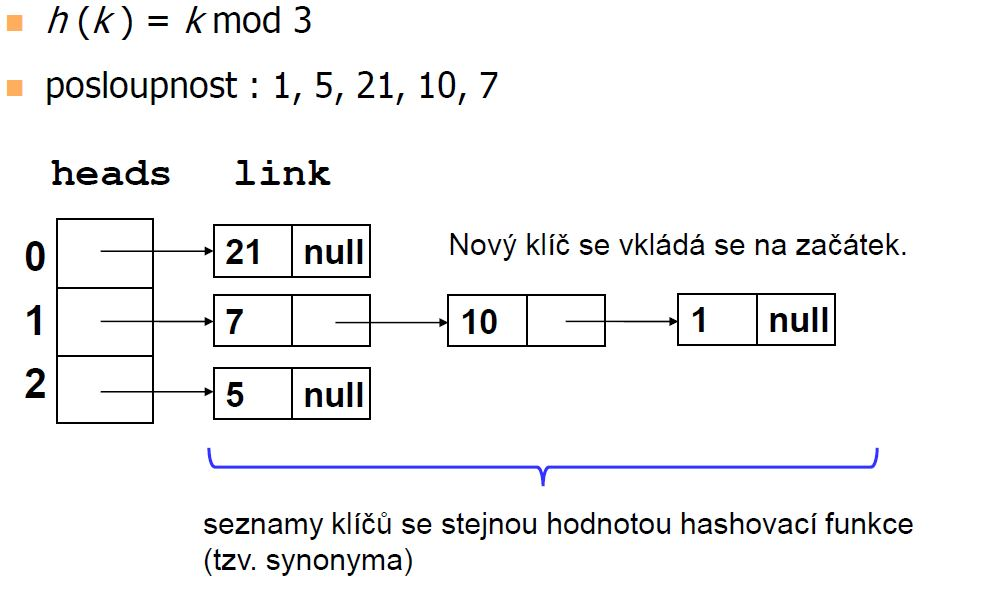
\includegraphics[width=12cm]{string.jpg}
\caption{Hashování se separovanými řetězci}
\label{fig:strings}
\end{center}
\end{figure}

\section{Otevřená hashování}

\begin{figure}[h]
\begin{center}
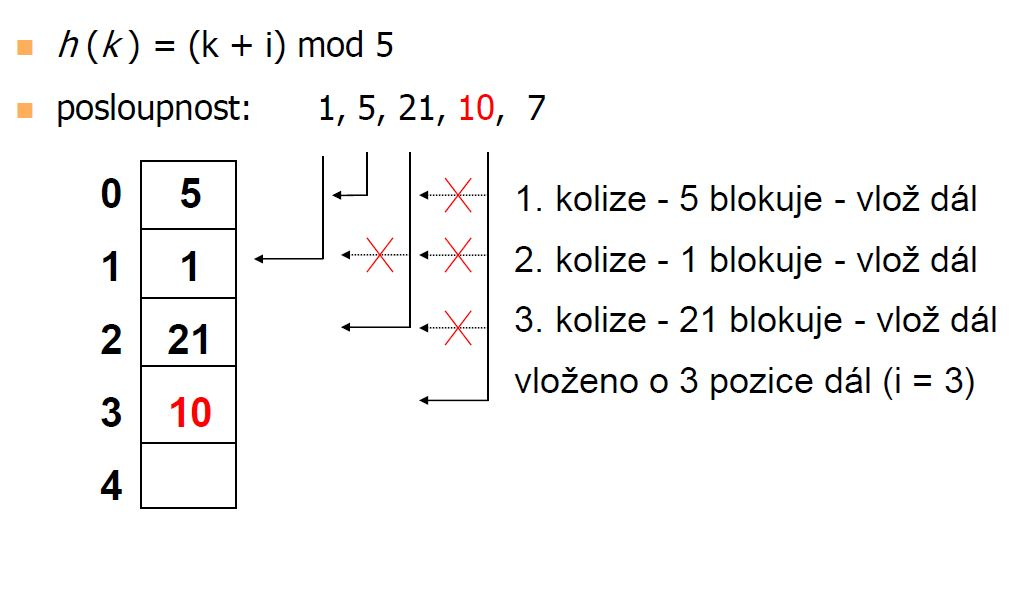
\includegraphics[width=12cm]{linear_probing.jpg}
\caption{Lineární přidávání}
\label{fig:linear_probing}
\end{center}
\end{figure}

\begin{figure}[h]
\begin{center}
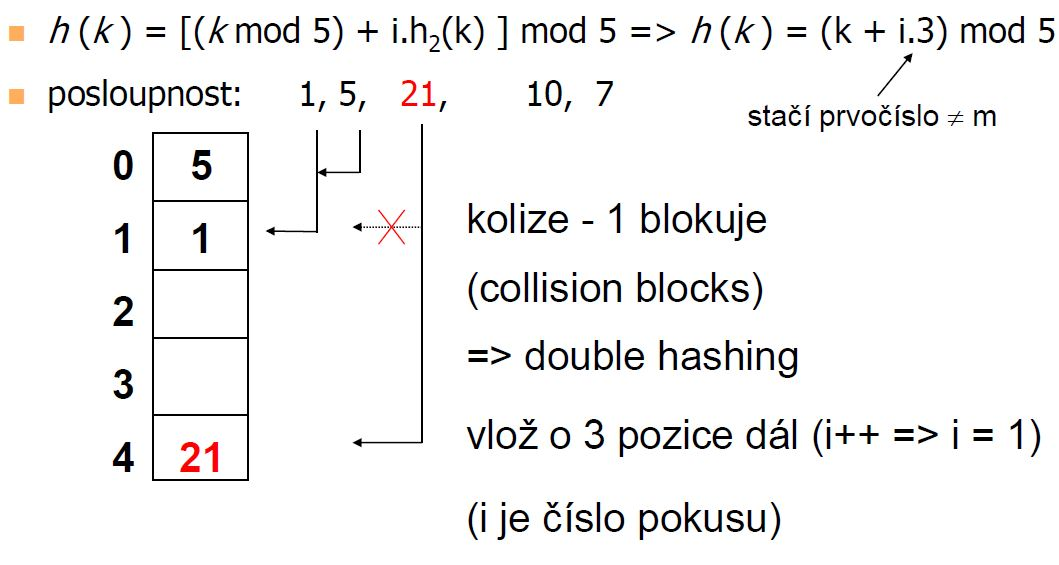
\includegraphics[width=12cm]{double_hashing.jpg}
\caption{Dvojité hashování}
\label{fig:double_hashing}
\end{center}
\end{figure}

\section{LISCH}

\begin{figure}[h]
\begin{center}
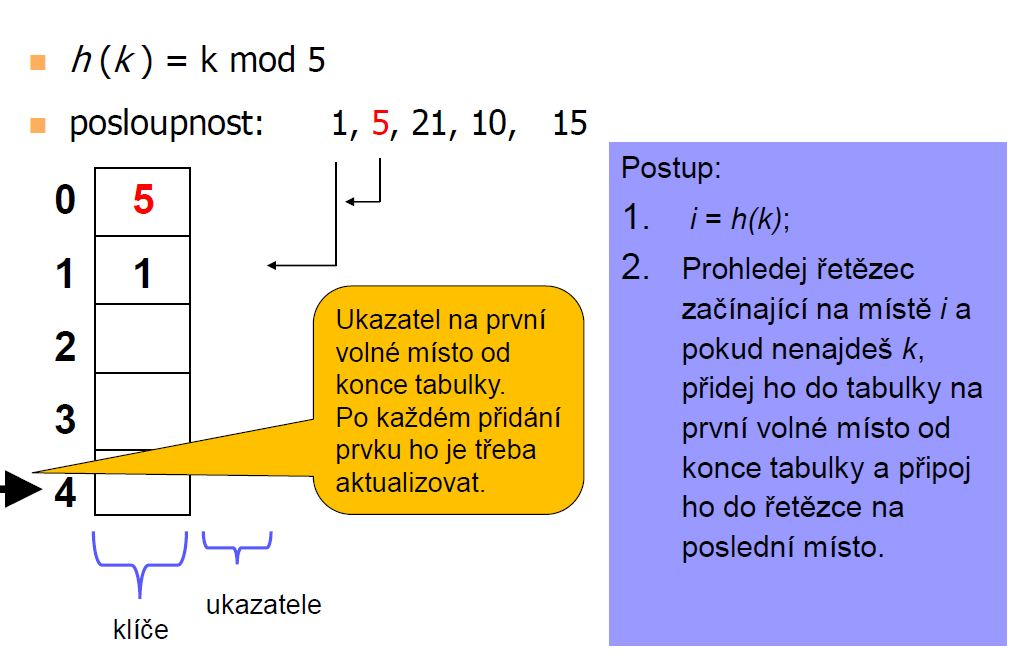
\includegraphics[width=12cm]{LISCH1.jpg}
\caption{LISCH 1}
\label{fig:lisch1}
\end{center}
\end{figure}

\begin{figure}[h]
\begin{center}
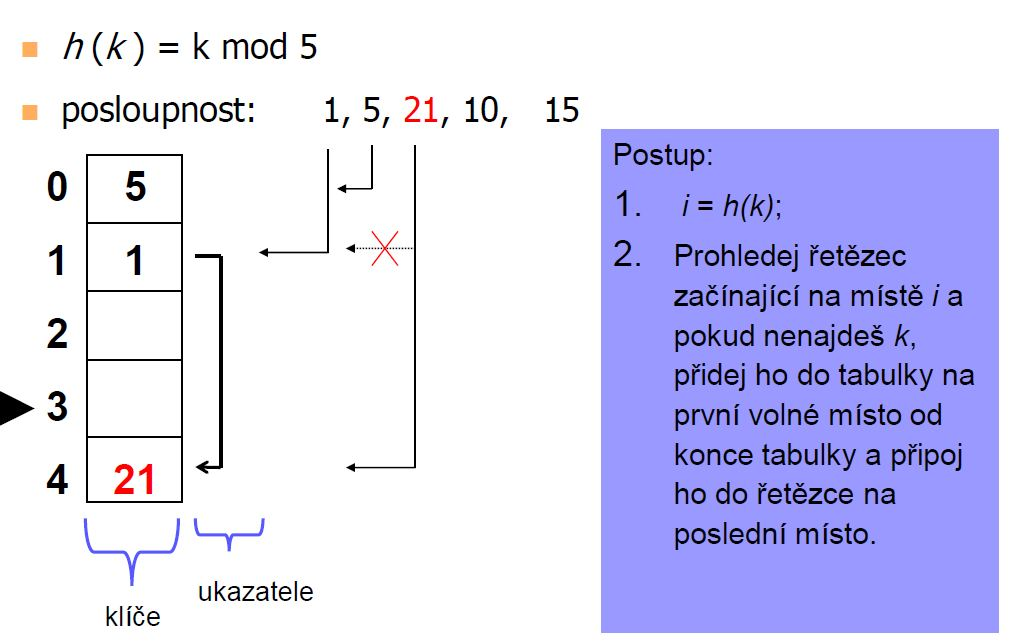
\includegraphics[width=12cm]{LISCH2.jpg}
\caption{LISCH 2}
\label{fig:lisch2}
\end{center}
\end{figure}

\begin{figure}[h]
\begin{center}
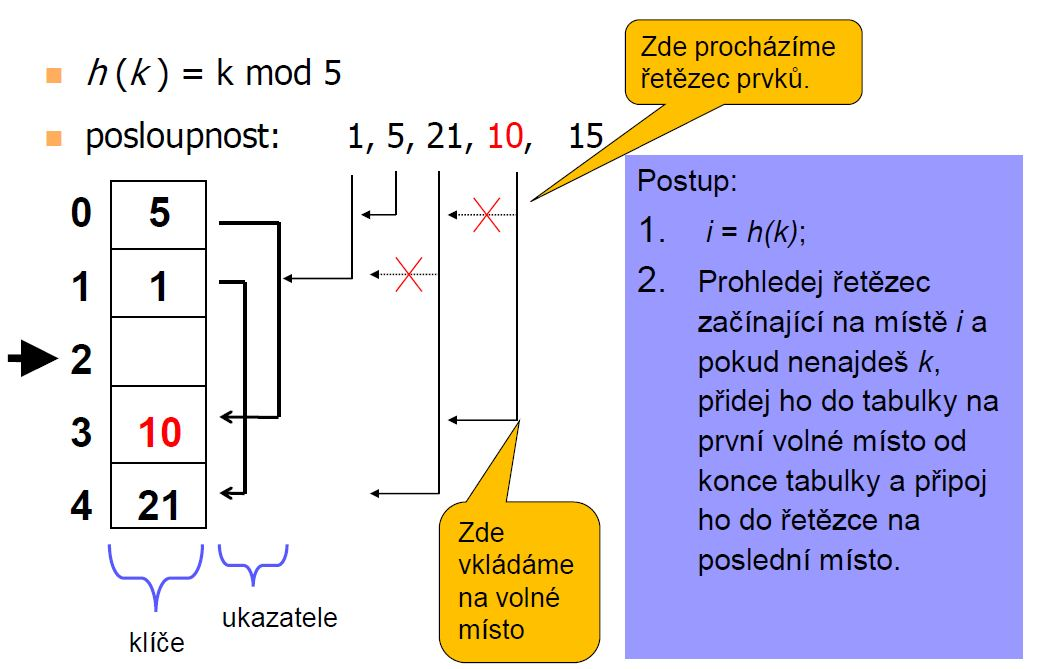
\includegraphics[width=12cm]{LISCH3.jpg}
\caption{LISCH 3}
\label{fig:lisch3}
\end{center}
\end{figure}

\begin{figure}[h]
\begin{center}
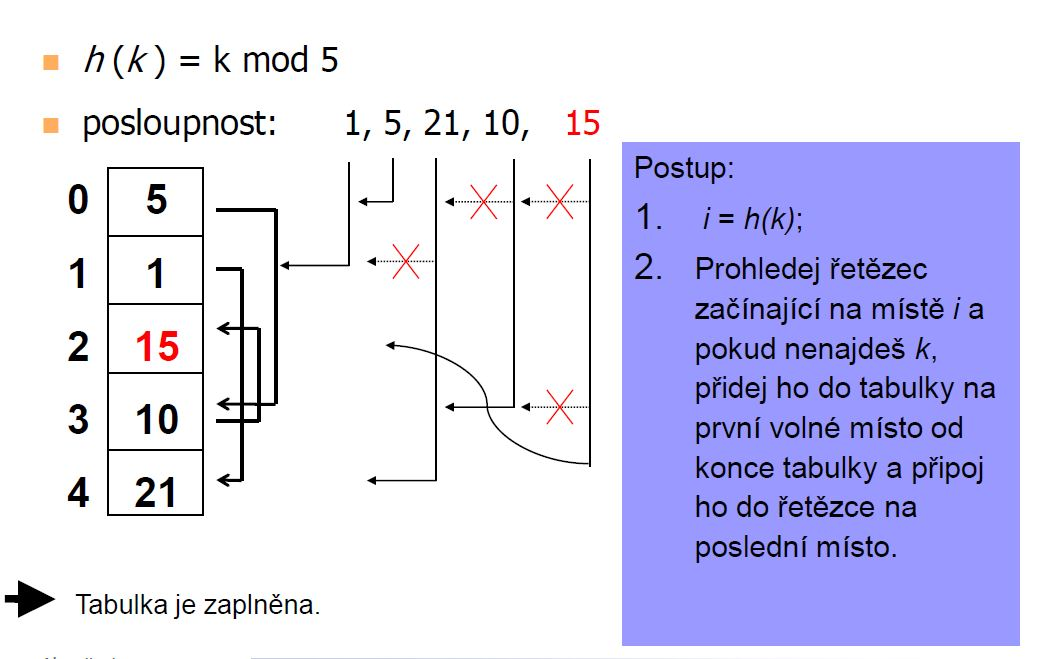
\includegraphics[width=12cm]{LISCH4.jpg}
\caption{LISCH 4}
\label{fig:lisch4}
\end{center}
\end{figure}

\section{EISCH}

\begin{figure}[h]
\begin{center}
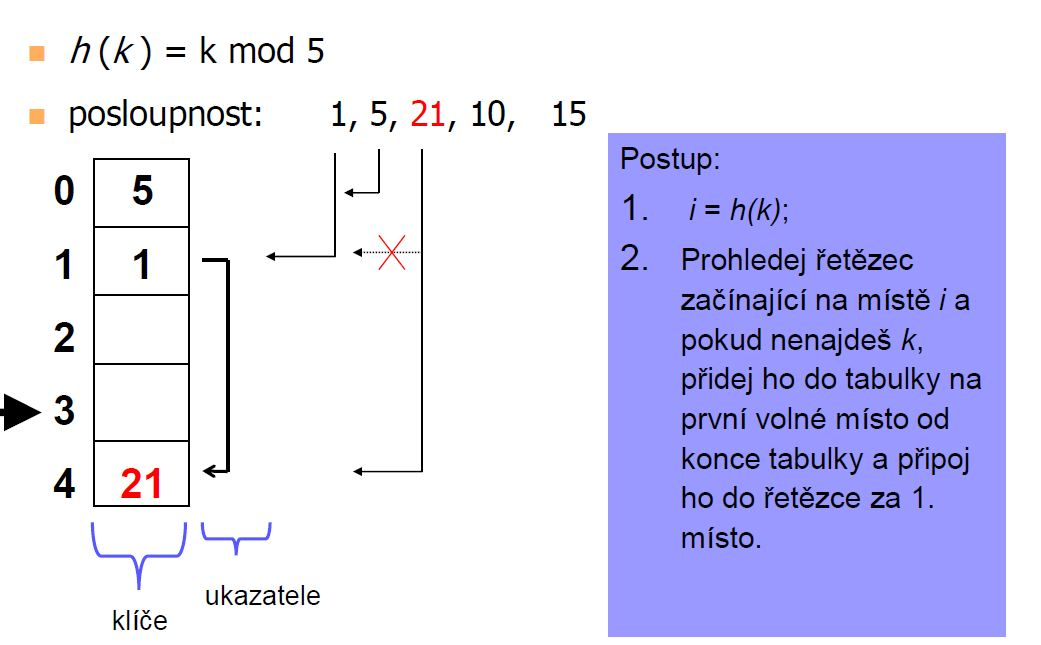
\includegraphics[width=12cm]{EISCH1.jpg}
\caption{EISCH 1}
\label{fig:eisch1}
\end{center}
\end{figure}

\begin{figure}[h]
\begin{center}
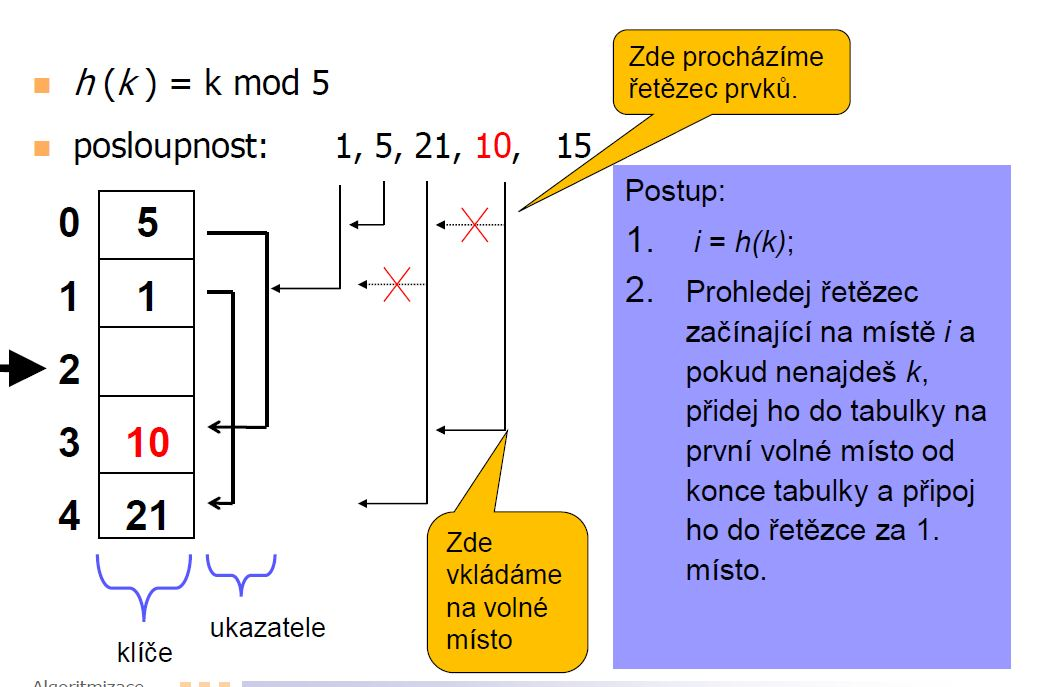
\includegraphics[width=12cm]{EISCH2.jpg}
\caption{EISCH 2}
\label{fig:eisch2}
\end{center}
\end{figure}

\begin{figure}[h]
\begin{center}
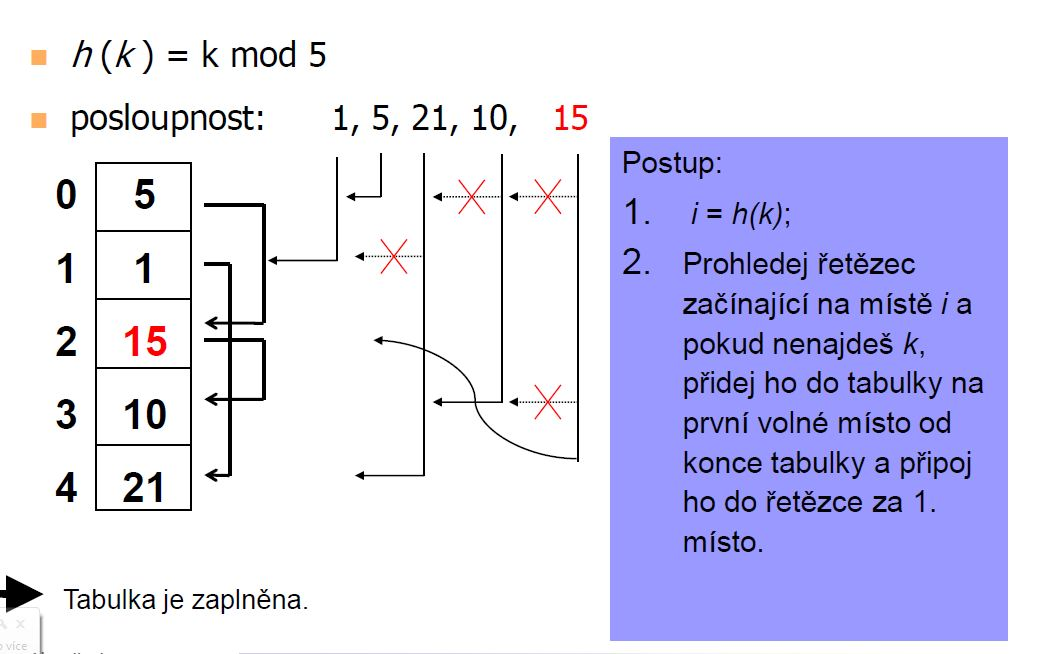
\includegraphics[width=12cm]{EISCH3.jpg}
\caption{EISCH 3}
\label{fig:eisch3}
\end{center}
\end{figure}

\section{LISCH vs EISCH}

\begin{figure}[h]
\begin{center}
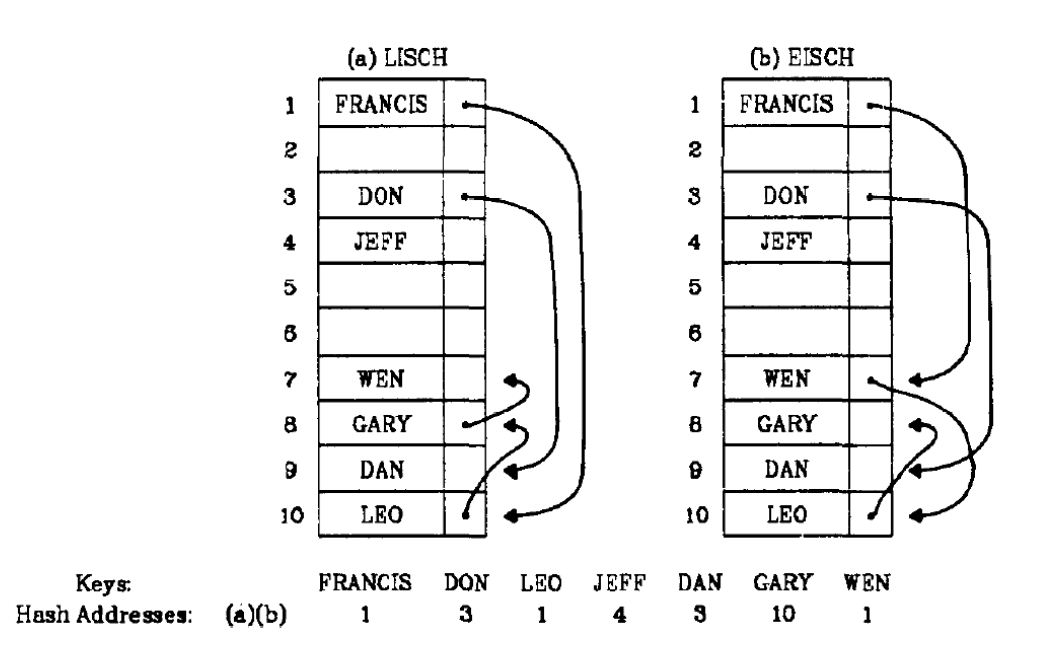
\includegraphics[width=12cm]{LISCHvsEISCH.jpg}
\caption{LISCH vs EISCH}
\label{fig:EISCHvsLISCH}
\end{center}
\end{figure}

\section{LICH vs EICH vs VICH}

\begin{figure}[h]
\begin{center}
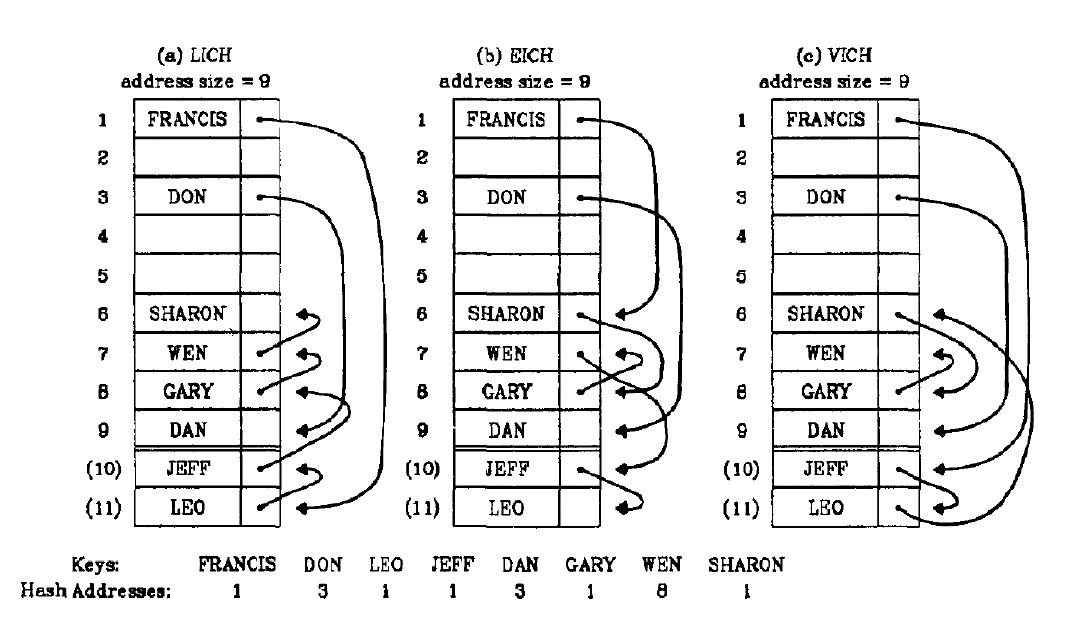
\includegraphics[width=12cm]{LICHvsEICHvsVICH.jpg}
\caption{LICH vs EICH vs VICH}
\label{fig:LICHvsEICHvsVICH}
\end{center}
\end{figure}

\end{document}